\documentclass[11pt]{report}
\usepackage[margin=2.5cm]{geometry}
\usepackage[french]{babel}
\usepackage[T1]{fontenc}
\usepackage[explicit]{titlesec}
\usepackage{times}
\usepackage{hyperref}
\usepackage{fancyhdr}
\usepackage{graphicx}
\usepackage{ucs}
\usepackage[utf8x]{inputenc}
\usepackage{awesomebox}
\usepackage{fontawesome5}
\setmainfont{Liberation Serif}

\titleformat{\chapter}[display]{\Huge}{\thechapter. #1}{20pt}{\small}

\titlespacing{\chapter}{0pt}{.1cm}{.1cm}

\lhead[\rightmark]{\rightmark}
\chead[]{}
\rhead[\thepage]{\thepage}

\lfoot[]{}
\cfoot[\thepage]{\thepage}
\rfoot[]{}

\renewcommand{\headrulewidth}{0.5pt}

\pagestyle{fancy}

\begin{document}
\begin{titlepage}
   \begin{center}
       \vspace*{5cm}

       \Huge\textbf{Manuel utilisateur}

       \vspace{0.5cm}
       \Large


       Moteur 3D - 7Physics


       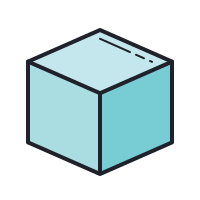
\includegraphics[width=2cm]{./logo.png}

       \vspace{1cm}

       \large
       \textbf{Équipe 3 : Noa AMMIRATI, Fanny DELNONDEDIEU, Quentin GENDARME, Pierre LOTTE, Théo PIROUELLE, Éléa TURC}

       \vfill

       
\includegraphics[width=15cm]{./enseeiht.jpeg}

       \vspace{2cm}

       ENSEEIHT\\
       Département Sciences du Numérique\\
       1APP SN 2020-2021


   \end{center}
\end{titlepage}


\tableofcontents

\chapter{Introduction}
L'objectif de ce manuel est de donner à l'utilisateur les bases nécessaires à la bonne utilisation de l'application.
L'application représente un moteur 3D permettant de réaliser des simulations de notions de physique élémentaires.
Un moteur 3D est un ensemble de fonctions permettant de représenter des objets dans un monde 3D, permettant de les
manipuler et de les afficher. Un autre objectif d'un moteur 3D est la gestion des interactions avec l'environnement (forces appliquées). \newline \newline


Les principales fonctionnalités du moteur 3D sont :
\begin{itemize}
        \item L'affichage de formes 3D prédéfinies et personnalisables (cube, sphere)
        \item L'utilisation de la caméra (permettant de changer d'angles de vue)
        \item L'animation des différentes formes contenues dans la scène 3D.
\end{itemize}

\chapter{Présentation générale de l'application}
[Faire une magnifique capture d'écran décrivant la structure principale de l'application, les différentes parties de l'IHM, leur objectif]

\chapter{Manipuler des objets 3D}

\section{Ajouter un objet 3D}
Pour pouvoir ajouter un objet 3D sur la scène 3D, il faut sur la partie supérieur droite de l'interface, sélectionner la forme souhaitée.
\newline

\begin{center}
    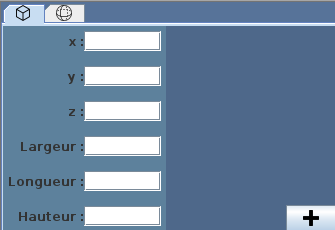
\includegraphics[width=5cm]{ajoutFormes}
\end{center}
\notebox{Pour afficher un \textbf{cube} sur la scène 3D, il faut sélectionner le bouton : 
\includegraphics[width=0.4cm]{./btn_cube.png}\newline
Pour afficher d'autres formes, il suffit de sélectionner les boutons adjacents. }


\chapter{Gestion de la caméra}

\warningbox{Afin de manipuler la caméra au clavier il est important de cliquer sur la scène en premier lieu. Sans cela, la caméra ne bougera pas.}

Afin d'observer la scène sous plusieurs angles, il est possible de manipuler la caméra. Les opérations possibles sont:
\begin{itemize}
        \item \hyperlink{zoom}{Zoomer}/\hyperlink{dezoom}{Dézoomer}
        \item \hyperlink{move}{Déplacements basiques (Gauche, droite, avant, arrière)}
        \item \hyperlink{moveV}{Se déplacer verticalement}
        \item \hyperlink{rotate}{Faire tourner la caméra.}
\end{itemize}

\section{Gestion du zoom}

Lors de la visualisation de la scène que vous avez créé, il vous est possible de régler le niveau de zoom utilisé afin de voir un objet plus en détail ou bien encore de voir une scène de taille importante en intégralité. Afin de réaliser ces actions, référez-vous aux explications suivantes.

\awesomebox{\faMousePointer}{3pt}{teal}{Attention, la gestion du zoom ne peut s'effectuer qu'à la souris.}

\subsection{Zoomer}

\hypertarget{zoom}{Il existe 2 possibilités pour zoomer sur la scène.}
\begin{itemize}
        \item La première est d'utiliser le bouton prévu à cet effet présent sur la gauche de votre écran représenté par ce symbole:.
        \item La seconde est d'utiliser la molette de votre souris en la faisant glisser vers le haut.
\end{itemize}

\subsection{Dezoomer}

\hypertarget{dezoom}{Il existe 2 possibilités pour dezoomer la scène.}

\begin{itemize}
        \item La première est d'utiliser le bouton prévu à cet effet présent sur la gauche de votre écran représenté par ce symbole:.
        \item La seconde est d'utiliser la molette de votre souris en la faisant glisser vers le bas.
\end{itemize}

\notebox{Afin de mieux maitriser votre environnement et de bénéficier d'une précision accrue, veuillez privilégier l'utilisation de la molette. En effet, les boutons latéraux sont limités à une manipulation prédéfinie du zoom et ne sont pas réglables.}


\section{Se déplacer sur la scène}

Afin de vous balader au sein de la scène pour visualiser celle-ci sous différents points de vue, il vous est possible de déplacer la caméra. Vous pourrez ainsi déplacer la caméra sur 3 axes différents que nous allons voir.

\awesomebox{\faKeyboard}{3pt}{teal}{Attention, les déplacememnts sur la scène ne peuvent être effectués que via le clavier et les raccourcis présentés.}

\subsection{Déplacements basiques}

\hypertarget{move}{Les premiers déplacement que nous allons voir sont les déplacements basiques gauche, droite, avant et arrière.} Ces déplacements se feront à l'aide des touches ZQSD du clavier.

\begin{itemize}
  \item \textbf{Z}: Avancer.
  \item \textbf{Q}: Se déplacer vers la gauche.
  \item \textbf{S}: Reculer.
  \item \textbf{D}: Se déplacer vers la droite.
\end{itemize}

\subsection{Déplacement vertical}

\hypertarget{moveV}{Ensuite, il peut être utile de bouger la caméra verticalement.} Pour cela, nous utiliserons les touches Espace et Shift.

\begin{itemize}
  \item \textbf{ESPACE}: Monter la caméra.
  \item \textbf{SHIFT}: Descendre la caméra.
\end{itemize}

\section{Tourner la caméra}

\hypertarget{rotate}{Enfin, pour finir, le dernier mouvement possible est la rotation de la caméra.} Pour cela, il suffit simplement de cliquer sur la scène 3D puis de glisser la souris vers l'endroit où vous souhaitez tourner la caméra en maintenant le clic de la souris.

\awesomebox{\faMousePointer}{3pt}{teal}{Attention, la rotation de la caméra ne peut se faire que via la souris.}

\chapter{Animer la scène 3D}

\section{Ajouter des forces}

\section{Lancer la simulation}

\end{document}
